\chapter{Inception: Requirements Capture}
\label{chap:inception}

\section{Introduction}

The inception phase turns the objectives of Chapter~\ref{chap:framework} into requirements. This chapter identifies the actors, states the functional and non functional requirements, builds the use case model that drives the iterations, lists the initial risks, and plans the work by phase and iteration.

\section{Actors}
\label{sec:actors}

An actor is a role played outside the system that interacts with it. CANvisionNative has three:

\begin{itemize}
    \item \textbf{Analyst (main actor).} A BMS engineer or tester who imports logs, starts replays and live sessions, reviews the alerts, asks for explanations, exports reports and configures the platform.
    \item \textbf{Vehicle or \gls{can} bus (secondary actor).} An external system that sends frames on the bus; it is the source of the traffic in a live session, through a \gls{can} adapter.
    \item \textbf{\gls{llm} provider (secondary actor).} An external service that writes the natural language text of an explanation: Google Gemini in the cloud, or a local Ollama model.
\end{itemize}

The backend of CANvisionNative is not an actor: it is part of the system under design, together with the desktop client.

\section{Functional requirements}
\label{sec:fr}

Table~\ref{tab:fr} groups the functional requirements by theme and gives each one a priority: \emph{must} for the requirements without which the platform has no purpose, \emph{should} for those expected in the final release, and \emph{could} for those that are useful but not essential.

\begin{table}[H]
\centering
\footnotesize
\caption{Functional requirements, by theme and priority.}
\label{tab:fr}
\begin{tabularx}{\textwidth}{|P{1.0cm}|Y|P{1.4cm}|}
\hline
\textbf{ID} & \textbf{Requirement} & \textbf{Priority} \\
\hline
\multicolumn{3}{|l|}{\textbf{Input and vehicle}} \\
\hline
FR1 & Import a recorded log in \gls{csv}, \gls{mf4}, Vector (.asc), candump (.log) or PCAN text (.txt) format, and convert it into one common frame stream made of a timestamp, an identifier and a payload. & Must \\
\hline
FR2 & Let the analyst choose the vehicle that produced the log, so that the matching trained model scores the frames and the matching \gls{dbc} file, when one exists, decodes them. & Must \\
\hline
FR12 & For a loaded log, show which signals it carries (the decoded signals when a \gls{dbc} file exists, otherwise the most active raw payload bytes, marked as not decoded) and describe the dataset: its size, its duration, and whether the selected model was trained or tested on it. & Should \\
\hline
FR13 & Show, for every vehicle model, whether it has been evaluated on a recording kept out of its training, and refuse an analysis with a model whose files cannot be shown to belong to one training run. & Must \\
\hline
\multicolumn{3}{|l|}{\textbf{Analysis}} \\
\hline
FR3 & Replay the imported frames in order, at a speed chosen by the analyst (0.5, 1, 2, 4 or 8 times real time, or 32 times as the maximum), and show the progress of the replay. & Must \\
\hline
FR4 & Score every frame for which a model exists and flag the frames whose score passes the calibrated threshold of that model; report the frames that cannot be scored as unresolved, with the reason, instead of counting them as normal; complement the model score with timing, payload and persistence checks. & Must \\
\hline
FR5 & Give each alert a severity level derived from its score. & Must \\
\hline
\multicolumn{3}{|l|}{\textbf{Explanation and reporting}} \\
\hline
FR6 & Explain any alert on request, in natural language, with the dominant signal, the likely cause and a recommended action. & Must \\
\hline
FR7 & Export the alert list as a \gls{csv} file and as a formatted PDF report. & Must \\
\hline
\multicolumn{3}{|l|}{\textbf{Live operation}} \\
\hline
FR8 & Generate a simulated live \gls{can} stream, including a simulated anomaly burst, to test the detection pipeline without a vehicle. & Could \\
\hline
FR9 & Connect to a physical \gls{can} adapter supported by python-can (for example a serial adapter using the slcan protocol, a PEAK PCAN adapter or SocketCAN) and send the received frames into the same runtime engine as replay; offer the live session only when a USB device is detected. & Should \\
\hline
FR10 & Record a live or simulated session to a log file, optionally with an injected and labelled anomaly, for later replay or training. & Could \\
\hline
\multicolumn{3}{|l|}{\textbf{Configuration}} \\
\hline
FR11 & Let the analyst set the key of the \gls{llm} provider, the hardware settings and an alert threshold, and keep these settings between sessions. & Should \\
\hline
\end{tabularx}
\end{table}

\section{Non functional requirements}
\label{sec:nfr}

Table~\ref{tab:nfr} classifies the non functional requirements with the \gls{furps} model.

\begin{table}[H]
\centering
\small
\caption{Non functional requirements, classified with FURPS+.}
\label{tab:nfr}
\begin{tabularx}{\textwidth}{|P{2.4cm}|P{1.1cm}|Y|}
\hline
\textbf{Category} & \textbf{ID} & \textbf{Requirement} \\
\hline
Usability & NFR3 & An analyst without a background in machine learning shall be able to import a log, read the alert list and understand the explanation of an alert without external documentation. \\
\hline
\multirow{2}{2.4cm}{Reliability} & NFR2 & A detection defect shall be shown and corrected with concrete evidence, never by tuning a threshold until the numbers look better. \\
\cline{2-3}
 & NFR6 & If the \gls{llm} provider cannot be reached, the system shall still produce a rule based explanation instead of failing. \\
\hline
Performance & NFR1 & An offline analysis of a recording of several hundred thousand frames shall finish in a few minutes on a standard desktop computer; live scoring shall keep up with the bus in real time. \\
\hline
\multirow{2}{2.4cm}{Supportability} & NFR4 & Every supported log format shall enter the detection pipeline through the same frame representation, so that the results do not depend on the format used to record the data. \\
\cline{2-3}
 & NFR5 & Adding a vehicle shall only require a \gls{dbc} file and a trained model folder that passes the promotion checks, without any change to the detection engine. \\
\hline
Constraints (+) & NFR7 & The desktop client shall run on Windows 10 or 11 with .NET Framework 4.8 and \gls{wpf}; the backend shall run as a local Python process (3.11 or later) that exposes a \gls{rest} \gls{api} on the same machine; only live capture needs extra hardware, a \gls{can} adapter supported by python-can. \\
\hline
\end{tabularx}
\end{table}

\Needspace{580pt}% keep the heading with its float
\section{Use case model}
\label{sec:usecases}

\subsection{Global use case diagram}

Figure~\ref{fig:usecase} shows the use case diagram. Replaying a log, running a live simulation and connecting the hardware include \emph{Detect anomaly}, because the three input modes feed the same runtime engine. Selecting a vehicle includes \emph{Check model status}, since a model is only used once its status allows it. \emph{Request explanation} is an optional extension of \emph{Review alerts}, and the only use case that involves the \gls{llm} provider.

\begin{figure}[H]
\centering
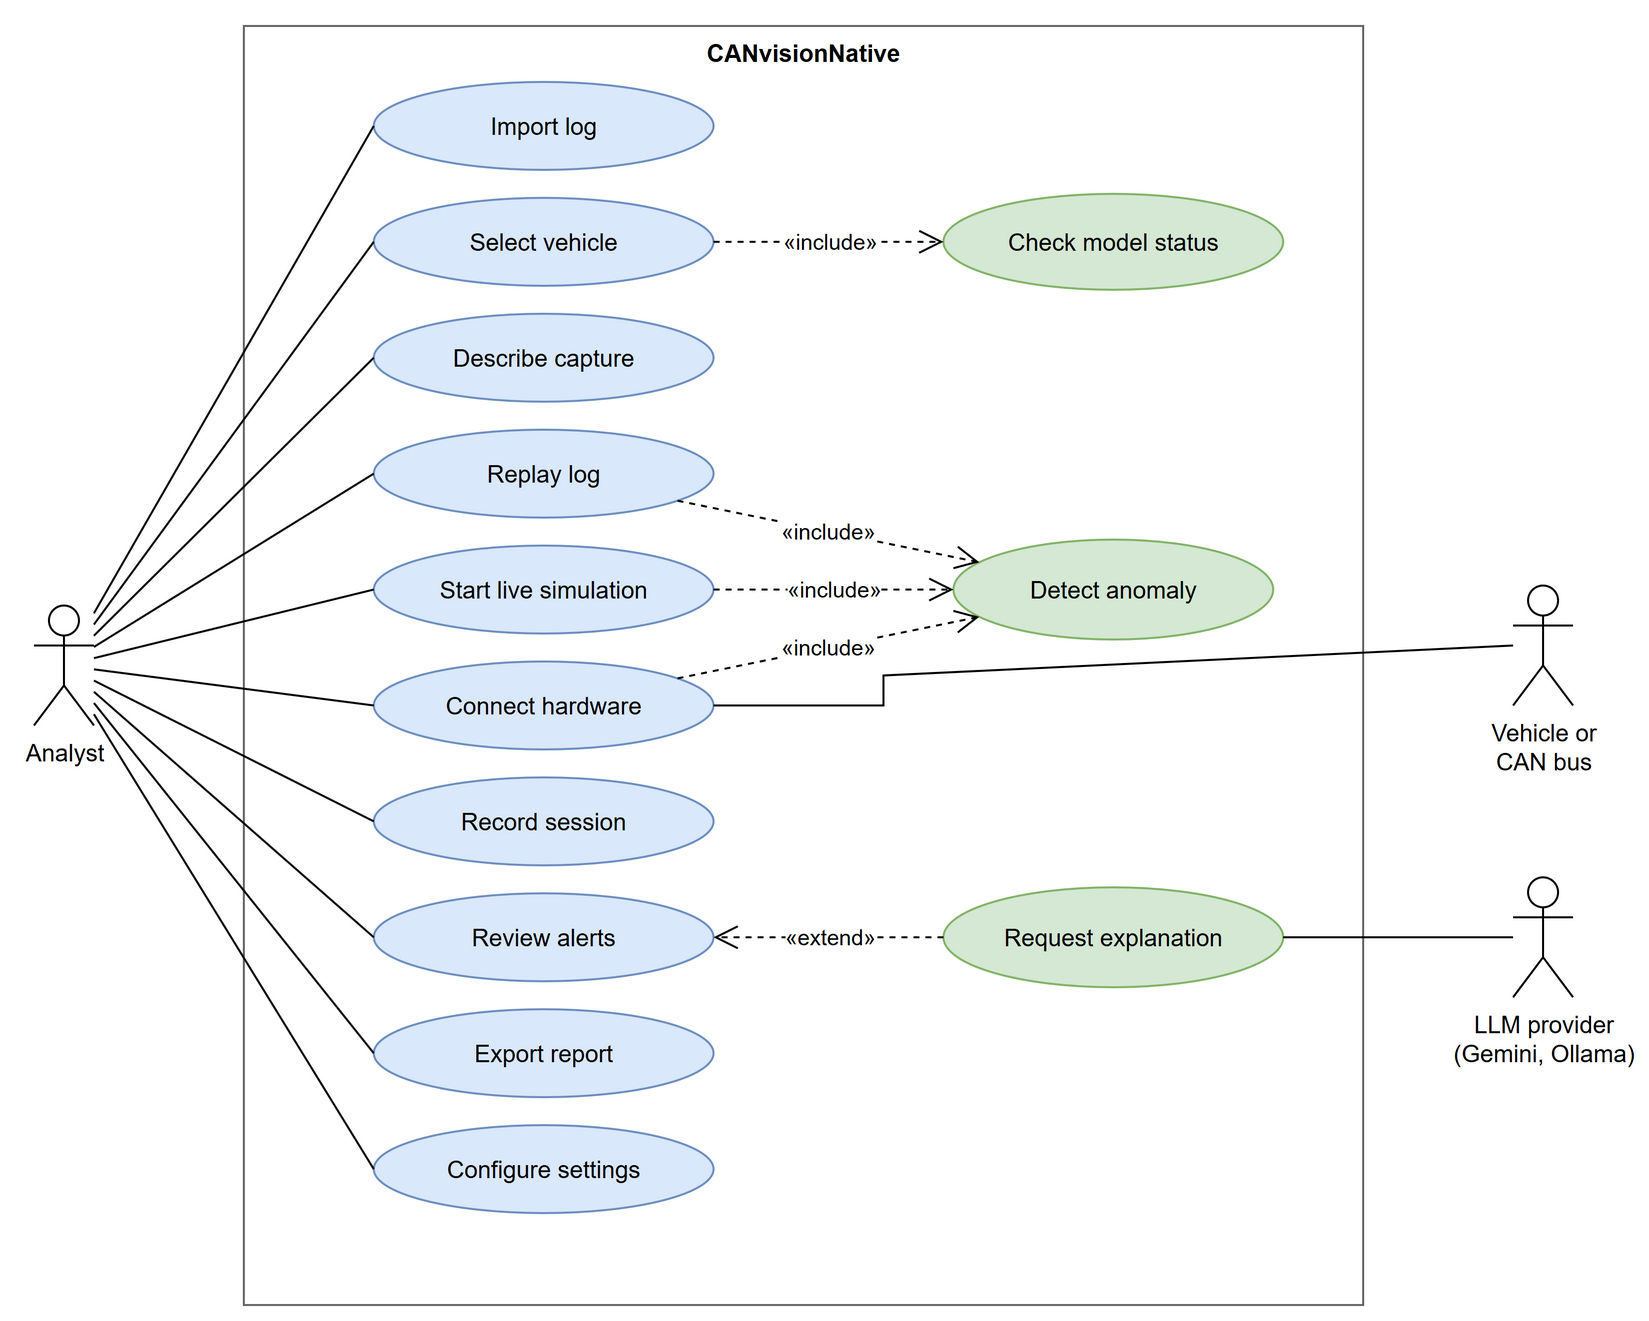
\includegraphics[width=\textwidth]{usecase.png}
\caption{Use case diagram of CANvisionNative.}
\label{fig:usecase}
\end{figure}

\Needspace{446pt}% keep the text with its float
Table~\ref{tab:usecase-table} summarises the use cases and the requirements they cover.

\begin{table}[H]
\centering
\small
\caption{Summary of the use cases.}
\label{tab:usecase-table}
\begin{tabularx}{\textwidth}{|P{3.3cm}|Y|P{1.7cm}|}
\hline
\textbf{Use case} & \textbf{Description} & \textbf{Req.} \\
\hline
Import log & The analyst selects a log file; the system recognises its format and converts it into the common frame stream. & FR1 \\
\hline
Select vehicle & The analyst chooses the vehicle model used to score the log and the \gls{dbc} file used to decode it. & FR2 \\
\hline
Check model status & The system tells whether the chosen model may be used offline or live, and refuses it otherwise. & FR13 \\
\hline
Describe capture & The system shows the signals of the capture and a plain description of the dataset. & FR12 \\
\hline
Replay log & The system replays the frame stream at the chosen speed and runs \emph{Detect anomaly} on it. & FR3 \\
\hline
Start live simulation & The system generates a simulated stream, with an optional anomaly burst, and runs \emph{Detect anomaly} on it. & FR8 \\
\hline
Connect hardware & The system reads live frames from a \gls{can} adapter and runs \emph{Detect anomaly} on them. & FR9 \\
\hline
Detect anomaly & The system scores each frame, reports the frames it cannot score, and raises alerts with a severity. & FR4, FR5 \\
\hline
Record session & The system records a live or simulated session to a log file. & FR10 \\
\hline
Review alerts & The analyst browses the alert list and the signals behind a selected alert. & FR4, FR5 \\
\hline
Request explanation & The system explains a selected alert in plain language. & FR6 \\
\hline
Export report & The analyst exports the alert list as a \gls{csv} file or a PDF report. & FR7 \\
\hline
Configure settings & The analyst sets the \gls{llm} key, the hardware parameters and the alert threshold. & FR11 \\
\hline
\end{tabularx}
\end{table}

\Needspace{395pt}% keep the heading with its float
\subsection{Textual descriptions}

Tables~\ref{tab:uc-analyse} to~\ref{tab:uc-hardware} describe the five main use cases in detail: their preconditions, nominal scenario, alternative scenarios and postconditions.

\newcommand{\ucrow}[2]{\textbf{#1} & #2 \\ \hline}

\Needspace{613pt}% keep the text with its float
Table~\ref{tab:uc-analyse} describes the offline analysis of a log: the use case \emph{Import log}, with the use cases \emph{Select vehicle}, \emph{Check model status} and \emph{Detect anomaly} that it includes.

\begin{table}[H]
\centering
\small
\caption{Use case \emph{Import log}, with \emph{Select vehicle}, \emph{Check model status} and \emph{Detect anomaly} (offline analysis).}
\label{tab:uc-analyse}
\begin{tabularx}{\textwidth}{|P{2.6cm}|Y|}
\hline
\ucrow{Actor}{Analyst.}
\ucrow{Preconditions}{The backend is running; a log file in a supported format is available.}
\ucrow{Nominal scenario}{1. The analyst chooses to import a log on the Home screen and selects a file. 2. The system recognises the format and reads the frames into the common frame stream. 3. The system lists the vehicle models with their status. 4. The analyst selects a model and starts the analysis. 5. The system checks that the model may be used offline. 6. The system scores every frame with the model of its identifier, counts the unresolved frames with their reasons, and merges bursts of alerts. 7. The system shows the results on the Dashboard.}
\ucrow{Alternative scenarios}{2a. The file cannot be read: the system shows the reason and the analysis does not start. 5a. The model may not be used offline (held back, not validated or from the first design): the system refuses the analysis with the reason, and the analyst can choose another model.}
\ucrow{Postconditions}{The alerts and the counts of the analysis are available to every screen of the client.}
\ucrow{Requirements}{FR1, FR2, FR4, FR5, FR13.}
\end{tabularx}
\end{table}

Table~\ref{tab:uc-replay} describes the use case \emph{Replay log}, which plays an imported log again through the runtime engine.

\begin{table}[H]
\centering
\small
\caption{Use case \emph{Replay log}.}
\label{tab:uc-replay}
\begin{tabularx}{\textwidth}{|P{2.6cm}|Y|}
\hline
\ucrow{Actor}{Analyst.}
\ucrow{Preconditions}{A log has been imported and a vehicle model selected.}
\ucrow{Nominal scenario}{1. The analyst opens Log Playback, chooses a speed and starts the replay. 2. The system starts a replay process that reads the file with the common parser. 3. The system sends every frame to the runtime engine (\emph{Detect anomaly}). 4. The client follows the progress and shows the flagged spans and the alerts on the timeline. 5. At the end of the file, the system publishes the alerts of the replay so that they can be explained.}
\ucrow{Alternative scenarios}{1a. The analyst pauses, resumes or stops the replay. 3a. A frame that no model can score is counted as unresolved, with its reason.}
\ucrow{Postconditions}{The replay is completed and its alerts are in the alert list.}
\ucrow{Requirements}{FR3, FR4, FR5.}
\end{tabularx}
\end{table}

\Needspace{535pt}% keep the text with its float
Table~\ref{tab:uc-explain} describes the use case \emph{Request explanation}, the only one that involves the \gls{llm} provider.

\begin{table}[H]
\centering
\small
\caption{Use case \emph{Request explanation}.}
\label{tab:uc-explain}
\begin{tabularx}{\textwidth}{|P{2.6cm}|Y|}
\hline
\ucrow{Actors}{Analyst; \gls{llm} provider.}
\ucrow{Preconditions}{An analysis or a replay has produced alerts, which the analyst reviews in Anomaly Intel.}
\ucrow{Nominal scenario}{1. The analyst selects an alert. 2. The system finds the alert in the current session and builds its context. 3. The system sends the context to Gemini. 4. Gemini returns a text. 5. The system shows the summary, the likely cause and the recommendation, with the name of the engine that wrote them.}
\ucrow{Alternative scenarios}{2a. The alert does not belong to the current session: the system returns no explanation. 3a. Gemini cannot be reached: the system asks the local Ollama model. 3b. No language model answers: the system writes a rule based text from the measured values.}
\ucrow{Postconditions}{The explanation is shown; the score, the flag and the severity of the alert are unchanged.}
\ucrow{Requirements}{FR6, NFR6.}
\end{tabularx}
\end{table}

Table~\ref{tab:uc-export} describes the use case \emph{Export report}, which saves the alert list of a session.

\begin{table}[H]
\centering
\small
\caption{Use case \emph{Export report}.}
\label{tab:uc-export}
\begin{tabularx}{\textwidth}{|P{2.6cm}|Y|}
\hline
\ucrow{Actor}{Analyst.}
\ucrow{Preconditions}{An alert list is shown in Anomaly Intel.}
\ucrow{Nominal scenario}{1. The analyst chooses to export the list as a PDF report or a \gls{csv} file. 2. The system asks for a file name. 3. The system writes the PDF report (session, summary by severity, identifiers with the most alerts, alerts in time order and explanations) or the \gls{csv} file (one row per alert).}
\ucrow{Alternative scenarios}{2a. The analyst cancels: nothing is written.}
\ucrow{Postconditions}{The report or the file is saved where the analyst chose.}
\ucrow{Requirements}{FR7.}
\end{tabularx}
\end{table}

\Needspace{304pt}% keep the text with its float
Table~\ref{tab:uc-hardware} describes the use case \emph{Connect hardware}, which starts a live capture from a \gls{can} adapter.

\begin{table}[H]
\centering
\small
\caption{Use case \emph{Connect hardware} (live capture).}
\label{tab:uc-hardware}
\begin{tabularx}{\textwidth}{|P{2.6cm}|Y|}
\hline
\ucrow{Actors}{Analyst; vehicle or \gls{can} bus.}
\ucrow{Preconditions}{The backend is running and a USB \gls{can} adapter is plugged in.}
\ucrow{Nominal scenario}{1. The analyst starts a live session on the Home screen. 2. The system opens the hardware setup. 3. The analyst chooses the interface, the port, the bitrate and the vehicle model, and connects. 4. The system builds a live engine for the chosen model and opens the adapter. 5. The system decodes each received frame with the \gls{dbc} file of the vehicle, when there is one, and scores it (\emph{Detect anomaly}). 6. The live screens show the signals and the alerts. 7. The analyst disconnects and the scoring stops.}
\ucrow{Alternative scenarios}{1a. No USB device is detected: the live session stays locked. 4a. The model is held back or unknown: the connection is refused with the reason. 5a. No frame arrives for a few seconds: the link is reported as lost.}
\ucrow{Postconditions}{The adapter is released; the alerts of the session remain available.}
\ucrow{Requirements}{FR2, FR9.}
\end{tabularx}
\end{table}

\Needspace{445pt}% keep the text with its float
\Needspace{431pt}% keep the heading with its float
\subsection{Activity diagram}

Figure~\ref{fig:activity-replay} shows the flow of the main use case, from the import of a log to the display of its results and their replay.

\begin{figure}[H]
\centering
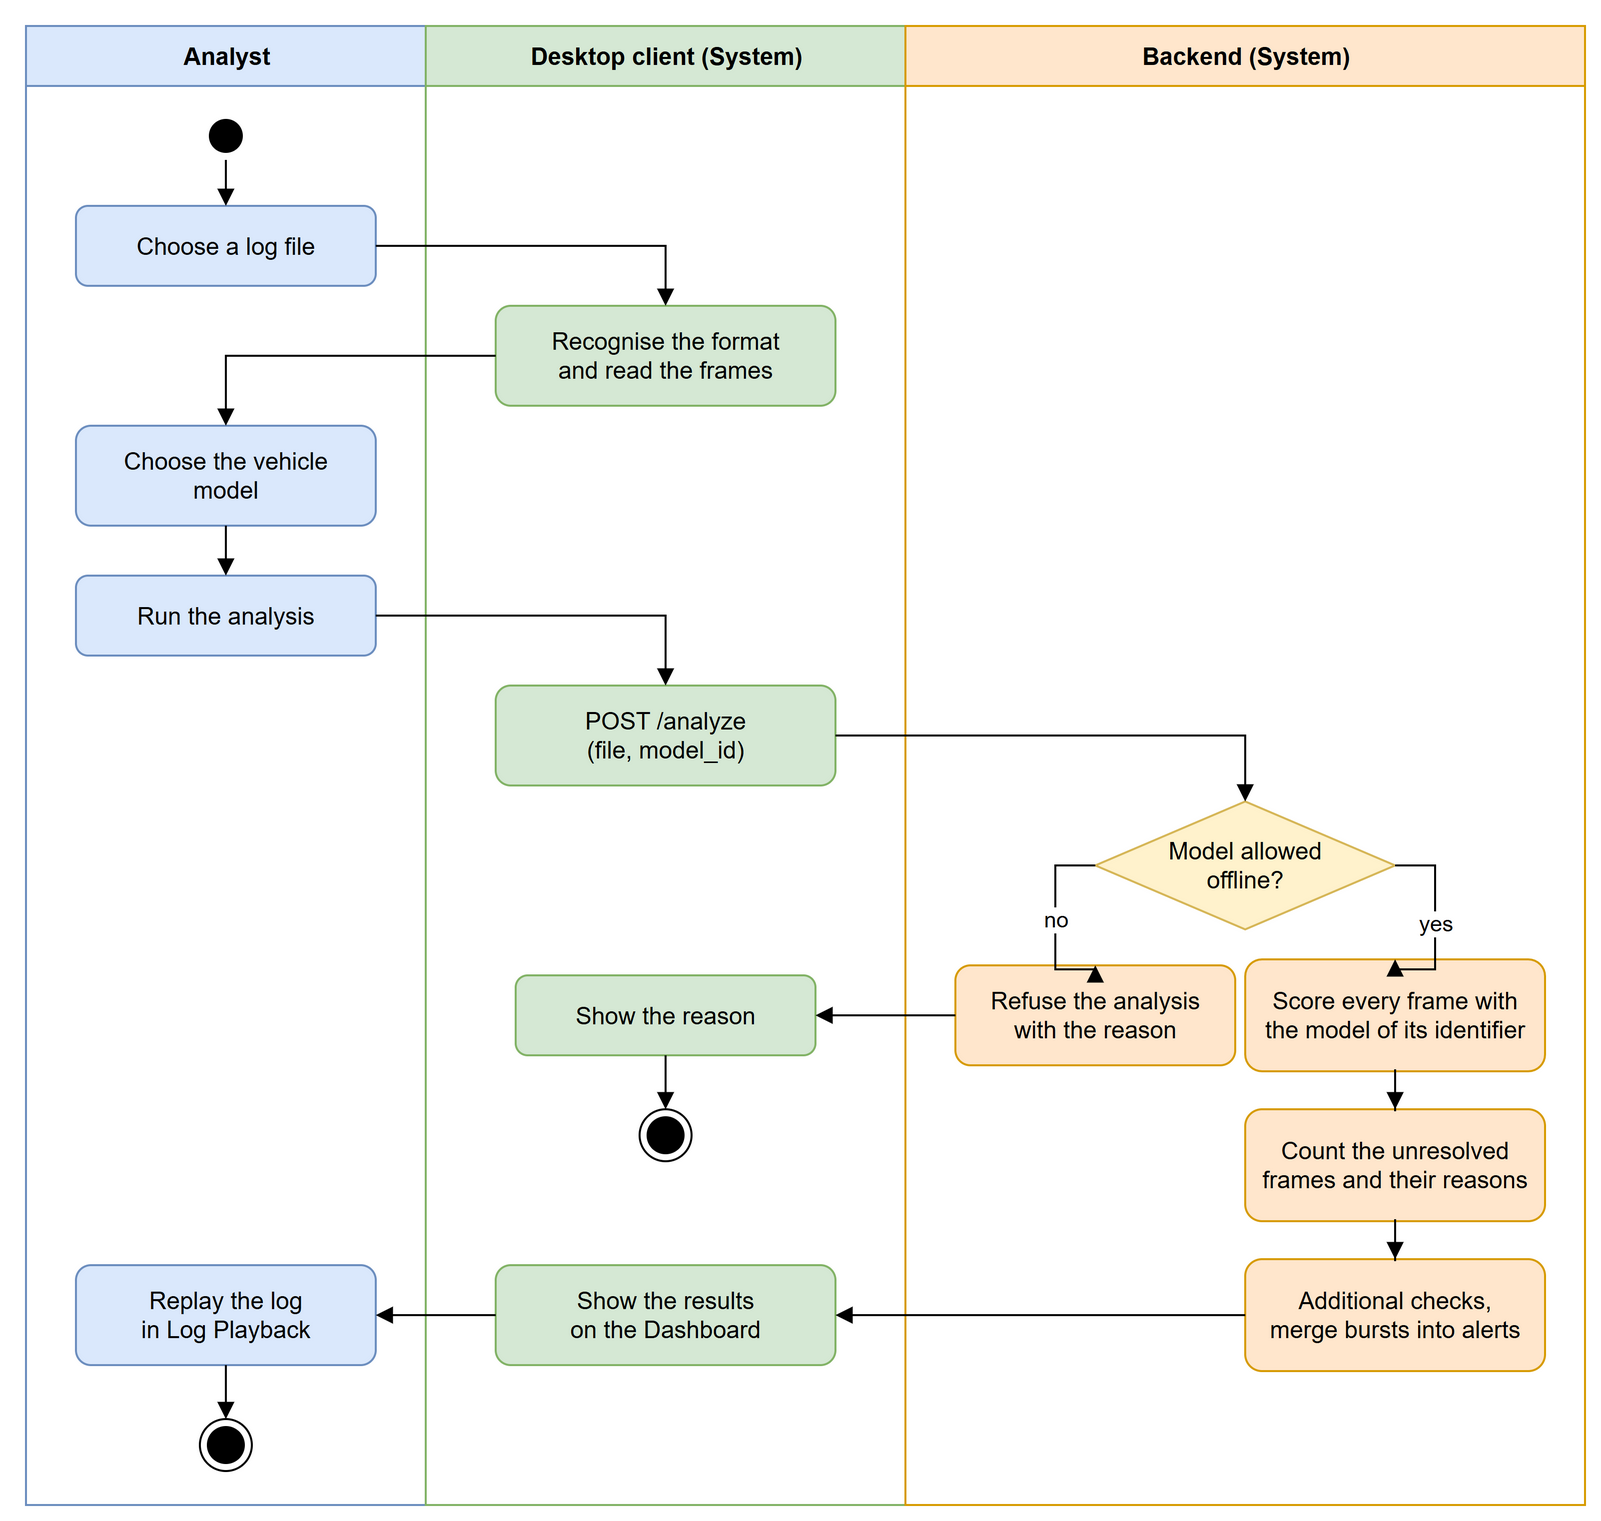
\includegraphics[width=0.74\textwidth]{activity_replay.png}
\caption{Activity diagram: importing, analysing and replaying a log.}
\label{fig:activity-replay}
\end{figure}

\Needspace{632pt}% keep the text with its float
\Needspace{622pt}% keep the heading with its float
\section{Initial risk list}
\label{sec:risks}

Table~\ref{tab:risks} lists the risks identified during inception, with their probability, their impact, the planned mitigation and the iteration that addresses each one. Following the \gls{up}, the iterations were ordered so that the riskiest parts were tackled early; what actually happened to each risk is discussed in the general conclusion.

\begin{table}[H]
\centering
\small
\caption{Initial risk list.}
\label{tab:risks}
\begin{tabularx}{\textwidth}{|P{3.0cm}|P{1.85cm}|P{1.3cm}|Y|P{2.05cm}|}
\hline
\textbf{Risk} & \textbf{Probability} & \textbf{Impact} & \textbf{Planned mitigation} & \textbf{Iteration} \\
\hline
R1. No vehicle available to test live capture & High & Medium & One runtime engine shared by replay, simulation and live capture, so that live capture differs only by its transport; a bench rig to test that transport. & Elaboration, iteration 3 \\
\hline
R2. \gls{llm} provider unavailable or not authenticated & Medium & Low & A chain of providers: Gemini, then a local Ollama model, then a rule based text. & Iteration 1 \\
\hline
R3. Wrong model applied to a vehicle & Medium & High & An explicit choice of the model, checked end to end on a real recording. & Iterations 2 and 4 \\
\hline
R4. A model that does not generalise to new recordings & Medium & High & Evaluate every model on a recording kept out of its training before it enters production. & Iteration 4 \\
\hline
R5. Live scoring too slow for buses with a high frame rate & Medium & Medium & An offline analysis path for whole recordings; measure the throughput of the live path. & Iteration 4 \\
\hline
R6. Too many alerts, so the analyst stops trusting them & Medium & High & Thresholds calibrated on the training data, persistence checks, and unscored frames reported apart instead of counted. & Iterations 2 and 4 \\
\hline
R7. Log formats read differently by different paths & Medium & Medium & One common parser and one frame representation for every path. & Iterations 1 and 2 \\
\hline
R8. Explanation shown for the wrong alert & Low & High & Tie each explanation to the alert of the current session, and test explanations across datasets of different vehicles. & Iteration 2 \\
\hline
\end{tabularx}
\end{table}

\section{Project plan by phase and iteration}
\label{sec:plan}

Figure~\ref{fig:gantt} shows the plan of the project from February to October 2026, organised by phase of the \gls{up}. The whole project was carried out alongside a full time QA position in the BMS team. Inception took the first week of February, while the work on the executable architecture of M1 was starting; the boundaries of the other periods also overlap slightly, because a milestone was being finished while the next one was starting.

\begin{figure}[H]
\centering
\resizebox{\textwidth}{!}{%
\begin{ganttchart}[
    time slot format=isodate,
    hgrid,
    vgrid=false,
    bar/.append style={fill=cyan!60},
    group/.append style={fill=black!70},
    bar height=0.6,
    group height=0.35,
    bar label font=\small,
    group label font=\small\bfseries,
    title label font=\small,
    y unit chart=0.62cm,
    y unit title=0.6cm,
    x unit=0.055cm
]{2026-02-01}{2026-10-31}
\gantttitlecalendar{month=shortname} \\
\ganttgroup{Inception}{2026-02-01}{2026-02-07} \\
\ganttbar{Vision, use cases, risks, plan}{2026-02-01}{2026-02-07} \\
\ganttgroup{Elaboration}{2026-02-02}{2026-03-13} \\
\ganttbar{M1: live foundation (architecture)}{2026-02-02}{2026-03-13} \\
\ganttgroup{Construction, iteration 1}{2026-03-02}{2026-06-22} \\
\ganttbar{M3: training for several driving states}{2026-03-02}{2026-04-24} \\
\ganttbar{M4: explanation engine}{2026-04-06}{2026-06-19} \\
\ganttbar{M5: real time charts}{2026-05-04}{2026-06-18} \\
\ganttbar{M6: session recording}{2026-05-25}{2026-06-21} \\
\ganttbar{M8: offline and live decoding}{2026-05-18}{2026-06-22} \\
\ganttbar{M7: integration}{2026-06-08}{2026-06-22} \\
\ganttgroup{Construction, iteration 2}{2026-06-22}{2026-07-31} \\
\ganttbar{Validation on real data}{2026-06-22}{2026-07-17} \\
\ganttbar{Correction and new validation}{2026-07-06}{2026-07-31} \\
\ganttgroup{Construction, iteration 3}{2026-08-10}{2026-09-12} \\
\ganttbar{M2: hardware layer and bench rig}{2026-08-10}{2026-09-12} \\
\ganttgroup{Construction, iteration 4}{2026-09-14}{2026-09-26} \\
\ganttbar{Model rebuild and holdout evaluation}{2026-09-14}{2026-09-26} \\
\ganttgroup{Transition}{2026-09-21}{2026-10-16} \\
\ganttbar{Final tests, deployment guide, report}{2026-09-21}{2026-10-16}
\end{ganttchart}%
}
\caption[Project plan by phase and iteration, February to October 2026.]{Project plan by phase and iteration of the Unified Process, February to October 2026 (Gantt chart).}
\label{fig:gantt}
\end{figure}

\section{Conclusion}

The inception phase identified three actors, thirteen functional and seven non functional requirements, the use cases that drive the iterations, and the main risks of the project. The next chapter presents the elaboration phase: the analysis and the architecture.
